\chapter{A Cellular Automata Model for Platoons}
\label{chapter:A Cellular Automata Model for Platoons}
The next section of the chapter presents a CA model for simulating the behavior of motorcyclists on the road. The section starts by identifying the essential requirements for the model, followed by the assumptions that underlie the model. The driving behavior of various road users is then described, including how the fun factor is defined for the motorcyclists and the concept of road curvature.

\section{Model Requirements}
\label{sec:Model Requirements}
The simulation model for this Bachelor's thesis have to meet the following requirements in order to accurately simulate the traffic for motorcycles in the Black Forest region:
\begin{itemize}
    \item The simulation model must account for mixed traffic as there are cyclists and cars to be expected on the road. 
    
    \item The vehicles in the simulation model should display a preference for the right lane of the road, and only use the left lane for overtaking other vehicles.
    \item The simulation model should allow for motorcyclists to be able to overtake slower vehicles and even other motorcyclists within the same platoon, if they are unable to fit into the queue properly, such as during an overtaking maneuver.
\end{itemize}

\section{Model Setup}
\label{sec:Model Setup}
The model setup fulfills the requirements in section \ref{sec:Model Requirements} and contains the following elements\footnote{see config.py file}:
\begin{itemize}
\item The simulation allows for three types of vehicles: Motorcyclists, cars and cyclists of variable quantity. This was chosen because cars are supposed to be faster than motorcyclists and cyclists are supposed to be slower, forcing them to adjust their driving behavior in a dense environment.
\item In keeping with the idea of cellular automata, all vehicles decide their own speed and lane changes. The vehicles update their behavior sequentially at each time step. See section \ref{sec:Model Update Behaviour} for more information. The "ping-pong" lane changes caused by tailgating described in Rickert et al.\cite{RICKERT1996534} should be significantly reduced.
\item The two-lane road is modeled with a list of tuples, where the tuple contains two elements representing the left and right lanes. The size of the road can be variable in length and only allows one direction\footnote{It is worth noting that bikes are not permitted on roads with multiple lanes in the same direction, which was not taken into consideration.}. The road is wrapped, which means it is a closed system with periodic boundary conditions. 
\item Time is modeled after each vehicle has made its driving decision and is moved forward on the road accordingly.
\item Speed is modeled as an integer representing how many tiles a vehicle moves forward on the road in the current time step.
\item The smallest section of a road is a tile. This is set to about 3m, which is about the length of a motorbike in a full traffic jam. This value corresponds to that suggested by Meng et al. \cite{MENG2007470}, who suggest 3.75m. Since the motorcyclist is supposed to ride in a platoon, a smaller value was chosen. Using the maximum speed of a car of 120 km/h, which is about 11 tiles/time step, one turn of the simulation represents one second in the real world, see equation \ref{eq:model_time_step}.
    \begin{align}
        3[\frac{m}{site}] * 11[\frac{sites}{time step}] / (120/3.6)[\frac{sec}{m}]\approx 1[\frac{sec}{time step}]
        \label{eq:model_time_step}
    \end{align}
\item A road has a maximum speed limit that depends on the curvature of the road. 
\item When the model is initialized, the vehicles are placed randomly, except for the platoon, which is always placed on the leftmost road in the left lane.
\item The focus lies on one platoon of motorcyclists. 
\end{itemize}

Figure \ref{fig:overtaking} shows a visual representation of the model setup where a platoon overtakes a slower cyclist. 

\begin{figure}[h]
    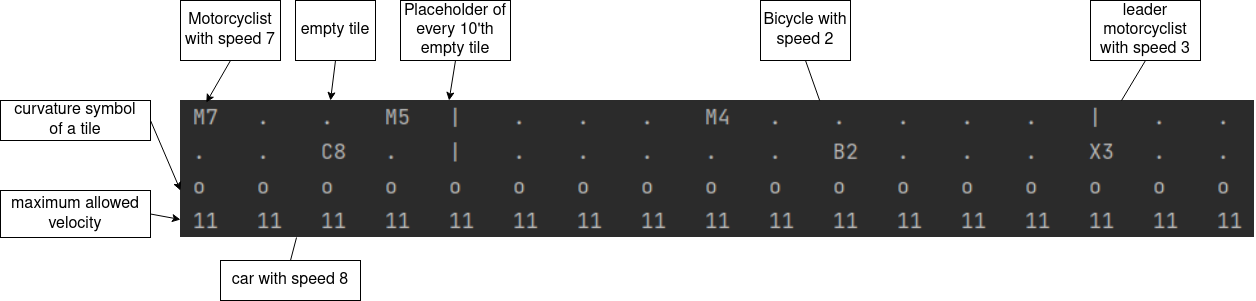
\includegraphics[width=1.0\linewidth]{images/overtaking.png}
    \caption{An overtaking maneuver of a platoon.}
    \label{fig:overtaking}
\end{figure}

In the simulation, the designations $M5, B2, C6$ are used to indicate the type and speed of the vehicles, with $M$ representing a motorcycle, $B$ a bicycle, and $C$ a car. The numerical value following each designation represents the speed of the respective vehicle. After the model update, which takes into account the movement of all vehicles, the visualization of traffic is displayed. To make the visualization easier, every tenth tile of the road is represented by a vertical bar (|), and the tilde symbol represents the road curvature. The first row represents the left lane and the second row represents the right lane of the road, with movement proceeding from left to right. The last line shows the maximum allowed speed of the tile.


 \section{Model Update Behavior}
 \label{sec:Model Update Behaviour}
This section presents the characterization of the driving behavior of each type of vehicle and outlines the process by which they are advanced within the simulation model. Figure \ref{fig:distanceExplained} provides a visual explanation of some of the key variables describing how far a vehicle can see in its surroundings.

\begin{figure}[h]
	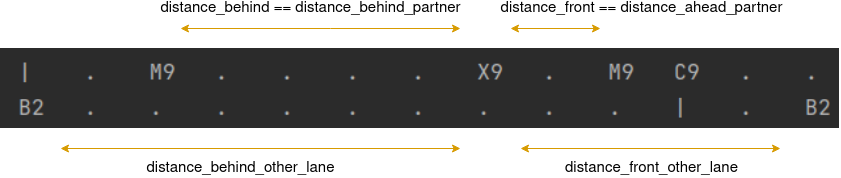
\includegraphics[width=1.0\linewidth]{images/distanceExplained.png}
	\caption{Visualization of distance variables for a motorcyclist marked as X. Since there are members of the same platoon in front and behind the motorcyclist, the variables distance\_behind equals distance\_behind\_partner and distance\_front equals distance\_ahead\_partner.}
	\label{fig:distanceExplained}
\end{figure}


 \begin{itemize}
     \item \textbf{Cars} \\
     The driving behavior of cars is primarily based on the model proposed by Rickert et al.\cite{RICKERT1996534}. In general, all cars aim to move forward at the highest possible speed.
     \begin{itemize}
         \item \textbf{Key Variables} \\
         - $distance\_front$: \\ 
         The clear distance in front of the vehicle in the same lane\\
         - $distance\_behind$: \\ 
         The clear distance behind the vehicle in the same lane\\
         - $distance\_front\_other\_lane$: \\
         The clear distance in front of the vehicle in the other lane\\
         - $distance\_behind\_other\_lane$: \\
         The clear distance behind the vehicle in the other lane\\
         - $speed$: \\
         The current velocity of the vehicle\\
         - $maxV$: \\
         The maximum velocity of the car, set to 9 tiles/time-step, which corresponds to 100 km/h\\
         
         \item \textbf{Update Speed Rule}
         \begin{enumerate}
             \item If there is enough free space in front of the car, taking into account a one-tile safety distance, and the car's current speed has not reached its maximum allowed velocity of $maxV$, the speed of the car will be increased [$v \rightarrow v + 1$]. This additional safety distance was included to account for the difference in length between a motorbike in a traffic jam and a car, as a tile is defined as 3m.
             \item If the distance in front, including a one-tile safety margin, is less than the current speed, decrease the speed by subtracting the value $[v \rightarrow v-j]$.
             \item The car's speed must not exceed the maximum allowed speed for the current tile it's on.
             \item If the $distance\_front$ in front is zero, the car must stop.
             \item There is a random chance that the car will slow down $[v \rightarrow v-1]$ by one. Note: This is disabled as it causes too much disruption to traffic.\\
         \end{enumerate}
         
         \item \textbf{Switching Lane Rule}
         \begin{enumerate}
         \item If the car is on the right lane it checks if the $distance\_front$ provides enough space even by increasing its speed from $[v \rightarrow v+1]$ .
         \item The car is only eligible to change lanes if the side is clear.
         \item The lane change is only executed if the $distance\_front\_other\_lane$ is greater than the current distance in front.
         \item Before changing lanes, the car checks the type of vehicle behind it on the other lane and its maximum speed. If the maximum speed of the other vehicle exceeds the $distance\_behind\_other\_lane$, the lane change is canceled to avoid blocking the other vehicle.
         \item If all of the above is true, then it will be decided at random whether the lane change maneuver will actually be carried out. Note: This is disabled as it causes too much disruption to traffic.
         \end{enumerate}     
     \end{itemize}

     \item \textbf{Bikes}
     \begin{itemize}
         \item \textbf{Key Variables}\\
         The key variables that influence the driving behavior of cyclists are the same as for cars.\\
         - $maxV$: \\
         The maximum velocity of the bike, which is set to 2 tiles/time-step, equivalent to 20 km/h.\\
         \item \textbf{Update Speed Rule}\\
         The update speed rule for a bike is similar to that of a car, adjusted to its maximum speed.\\
         \item \textbf{Switching Lane Rule}\\
         As the slowest participant in traffic, the bike will strive to move to the right lane as soon as it is randomly placed on the road and will remain there, even in congested traffic.
     \end{itemize}

     \item \textbf{Motorcycles}
     \begin{itemize}
         \item \textbf{Key Variables}\\
          The motorcycle class, as the primary object of study, is equipped with additional variables compared to cars. The motorcycles aim to maintain a formation as a line during the simulation and have a fixed preferred distance from their partners, as well as a preferred speed. Each biker is assigned a role as a sweeper, in-between, or leader. A partner is defined as a motorcycle that the rider can see directly in front of or behind them in either lane. \\
          - $moved$:\\
          A boolean value that indicates whether the driver has already updated their speed and is moving forward. This is crucial in the simulation, as each vehicle is updated in sequence.\\
          - $distance\_behind\_partner$:\\
          The distance from the motorcycle behind the rider. \\
          - $distance\_ahead\_partner$:\\
          The distance from the motorcycle in front of the rider. \\
          - $close\_up\_dist\_behind$ and $close\_up\_dist\_ahead$:\\
          These variables account for the fact that in the simulation, as each vehicle is updated in sequence, the motorcyclist cannot know exactly what speed their partner might choose for the current time step and how far away they will be in the next. The rider must make an estimate based on their current distance and speed, as well as the distance and speed of their partner, who may or may not have moved in the current time-step.\\
          - $preferred\_distance$:\\
          The preferred distance that a motorcyclist likes to keep from other motorcyclists in their platoon, either in front or behind. This is assumed to be 5 tiles, equivalent to 15 meters. Based on the "One Second Rule\footnote{https://www.quora.com/When-riding-a-motorcycle-in-group-formation-staggered-how-close-should-you-be-to-the-bikes-in-front-of-you, comment by Daniel Wallander, 10.02.23}", a 15 meter distance is considered optimal for a staggered formation traveling at 55 km/h. Unlike cars, there is no implemented safety distance for motorcyclists.\\
          - speed\_preference:\\
          The preferred speed of the motorcyclist, which is determined by the curvature of the current tile he is on. For more see section \ref{sec:Curvature definition and parameter calibration}\\
          - $is\_leader$, $is\_sweeper$, $is\_inbetween$:\\
          The leader is in front, the sweeper is at the back, and the in-between are those in the middle. Each rider can only have one role\footnote{The code has been designed to handle the case where a single driver gets lost and has no partner at all in the platoon. This situation has the potential to cause a runtime error, especially when simulating a large number of platoons or when the size of a platoon becomes too big. However, to date, no such errors have been encountered.}.\\
          - $fun$:\\
          A measure of how well the rider is able to maintain their preferred distance from other riders and how well they are able to ride at their preferred speed. For more see section \ref{sec:Fun Metric}\\
          - $maxV$:\\
          The maximum velocity of the motorcycle is set to 8 tiles per time-step, which corresponds to 85 km/h. While a motorcycle may have the ability to reach higher speeds, it is assumed that vehicles travel at a slower pace in the Black Forest region\footnote{This assumption has not been confirmed.}.\\
          

        \item \textbf{Update Speed Rule}
         \begin{enumerate}
             \item Observe the current location and distance from each respective partner.
             \item Estimate whether the preferred distance to the partner behind will be shorter or longer for the next time step when the speed is changed. The preferred distance to the partner behind has priority over the preferred distance to the partner in front, which is adjusted when the optimum distance to the partner behind has been achieved. In the case of the platoon leader or sweeper, they only need to monitor the distance to one rider.
             \item The minimum speed at which a motorcyclist is willing to slow down for the partner behind them is 3 tiles/time-step, equivalent to 30 km/h.
             \item When the optimum distance to each partner is reached, the speed is adjusted to their preferred speed according to the curvature of the road. This makes the leader of the platoon important, as he determines the speed dynamics of the group as well as the spatial compression of the platoon. 
             \item There is a random chance that the motorcyclist will reduce his speed by one. Note: This is mostly disabled as it causes too much disruption to traffic. 
         \end{enumerate}
         \item \textbf{Switching Lane Rule}\\
         The leader of the platoon is typically responsible for making lane switching decisions, with other members following behind. If there is already a platoon member directly in front, the decision will be bypassed.
         \begin{enumerate}
         \item The switching lane rule is applied asymmetrically. If the leader is on the left lane, it will attempt to switch to the right if there is sufficient space, without braking. If the leader is on the right lane, it will check if the $distance\_front$ is less than two times its current speed. When looking ahead for obstacles, the leader will consider a longer distance than a car, as the other platoon members need time to successfully follow the leader during an overtaking maneuver.
         \item Switching to another lane is only possible if the side is free. 
         \item Switching is only worthwhile if the $distance\_front\_other\_lane$ is greater than the current speed plus one. This additional buffer was added to discourage frequent lane switching and maintain the stability of the platoon.
         \item Switching is only possible if the $distance\_behind\_other\_lane$ is greater than the actual speed of the vehicle behind on the other lane. This approach makes motorcyclists more aggressive in lane changing, as compared to cars which consider the maximum speed. This enhances the stability and cohesion of the platoon.
         \item If all of the above is true, then it will be decided at random whether the lane change maneuver will actually be carried out. Note: This is disabled as it causes too much disruption to traffic.
         \end{enumerate}  
     \end{itemize}

     \item \textbf{Model update}\\
     The model updates at each time-step by following these steps:
     \begin{enumerate}
         \item Each vehicle determines its own speed.
         \item Each vehicle is moved forward in its current lane, based on its speed.
         \item Each vehicle decides whether to change lanes.
         \item Each vehicle is moved to a different lane depending on its previous decision.
     \end{enumerate}
 \end{itemize}

 \section{Curvature definition and parameter calibrations}
 \label{sec:Curvature definition and parameter calibration}
The definition and explanation of the curvature for a tile has been obtained from the website \hyperlink{}{www.roadcurvature.com}, which is authored and maintained by Adam Franco\cite{roadcurvature.com}.
This website uses data from OpenStreetMap\textsuperscript{\textcopyright}\footnote{\hyperlink{}{https://www.openstreetmap.de/}, 20.02.23} to provide information about road segments and their corresponding curvature values. The road curvature is highlighted on the map with a color coding scheme, offering users a visual representation of the curvature, with the data available through tooltips, see figure \ref{fig:tooltip}.

The idea is to calculate "the radius of curvature at at every segment of every road and then adding up the length of the most curvy segments to get a total distance spent cornering"\cite{roadcurvature.com}, see figure \ref{fig:radiicalculation}. The road is represented as a graph model on a map, with vertices connected by edges to form a line. A set of three points form a triangle that intersects all three points (with the exception of the edge case of a straight line). Each vertex is assigned a radius attribute based on the calculated triangle. If a vertex is connected to two other vertices, the curvature of the edge is the average of the radii of its neighboring vertices. The curvature of the line as a whole is calculated by summing the curvatures of its edges. "Since numbered highways may go hundreds or thousands of miles, only a portion of which are twisty, each road is subsequently split into sections if it goes more than two miles without any curves that push a segment out of the straight bucket. This splitting process allows twisty sections to be highlighted alone without their adjoining long straightaways\cite{roadcurvature.com}". The final step in the process involves assigning weights to the summarized radii-turns. Broad sweeping turns receive a weight of 1, tighter turns receive a weight of 2, and super tight corners receive a weight of 4. The resulting weighted sum of these segments represents the curvature value of the road.

\begin{figure}[h]
\centering
    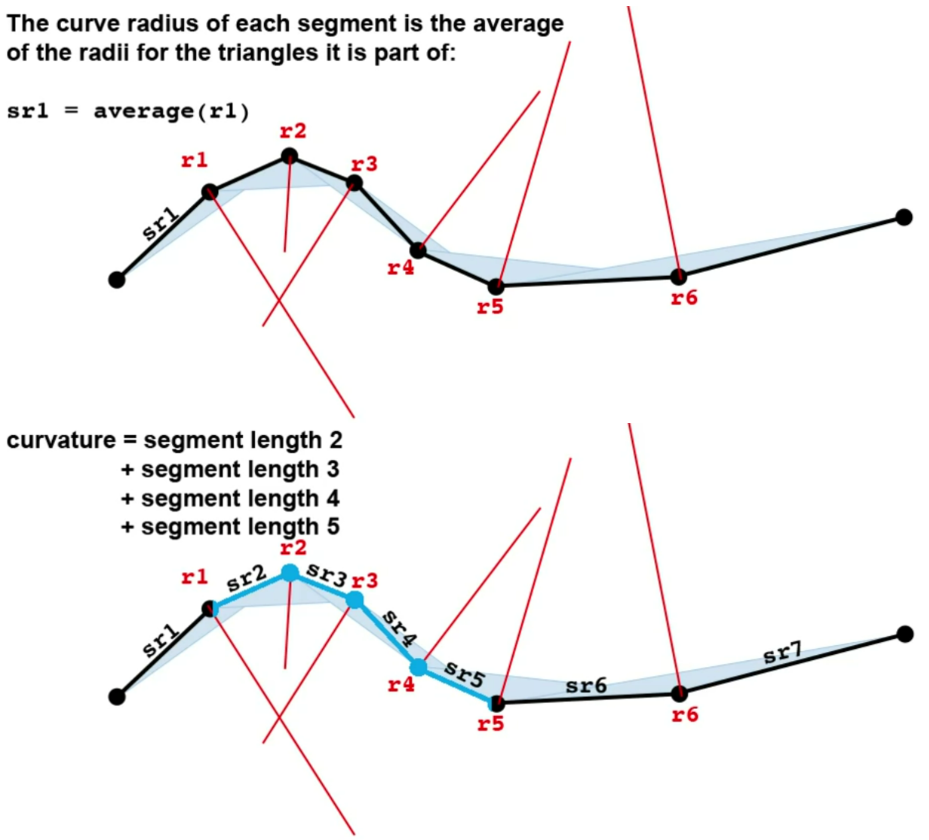
\includegraphics[width=0.8\linewidth]{images/radii.png}
    \caption{Curvature calculation taken from roadcurvature.com \cite{roadcurvature.com}.}
    \label{fig:radiicalculation}
\end{figure}

The curvature calculation algorithm considers the possibility of conflicts at intersections and crossings where merging traffic streams converge, as these roads may not be as fun to ride as similar roads with the same curvature. Further the algorithm "zeros-out the curvature rating for 30 meters in both directions from each conflict point along the roadway. By zeroing out curves near these conflict zones ... [the algorithm] can avoid suggesting roads that really aren't very fun\cite{roadcurvature.com}". This helps identify curvy roads in urban areas, but has little impact on the results in more rural areas, such as the Black Forest region.

The storage of road curvature geodata in Keyhole Markup Language (KML) format presents a challenge for utilization due to the need for a preliminary understanding of its schema. To overcome this, the necessary data was extracted manually from the tooltips provided in the in-browser map, rather than through automated crawling, see figure \ref{fig:tooltip}.

\begin{figure}
    \centering
    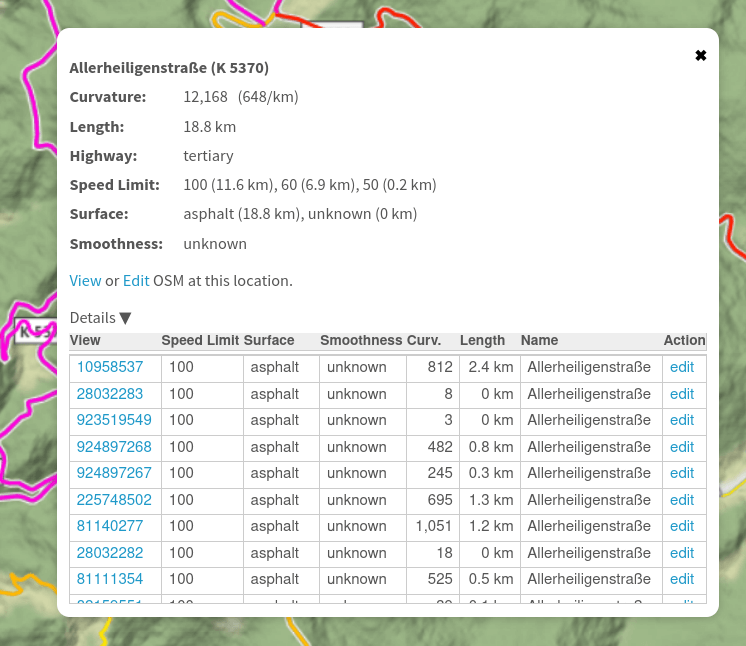
\includegraphics[width=0.8\linewidth]{images/tooltip.png}
    \caption{Tooltip for Allerheiligenstraße, source: roadcurvature.com, 20.02.23}
    \label{fig:tooltip}
\end{figure}

The seven roads randomly selected for the thesis are considered to have a high level of curviness, as indicated by their depiction as purple roads on the map. Those roads are listed in table \ref{tab:roadsample}

    \begin{table}
    \centering
    \begin{tabular}{@{}llr@{}} \toprule
        Name                                      & Sum Length [km] & Sum Curvature \\ \midrule
        Großherzog-Friedrich-Luisen-Straße (L 79) & 13              & 12106         \\
        Sandstraße (L83)                          & 21.8            & 8439          \\
        Allerheiligenstraße (K 5370)              & 18.8            & 12168         \\
        Wildschapbachstraße (L 93)                & 12.5            & 9488          \\
        Nordracher Straße (K 5354)                & 12.2            & 6290          \\
        Kaltenbronner Straße (L 76b)              & 18.9            & 6917          \\
        Rippoldsauer Straße (L 96)              & 29.9              & 11055         \\\bottomrule
    \end{tabular}
    \caption{Selected roads in the Black Forest from the in-browser map tooltips from roadcurvature.com} 
    \label{tab:roadsample}
    \end{table}

The \hyperlink{https://roadcurvature.com}{roadcurvature.com} website offers an overview to interpret the summarized curvature values. According to this overview:
\begin{itemize}
    \item A curvature value of less than 300 indicates a relatively straight road.
    \item A curvature value between 300 and 1000 suggests a road with several significant corners close together.
    \item A curvature value between 1000 and 3000 indicates a road with few dozen corners.
    \item A curvature value between 3000 and 10000 suggests a road with long sections of tight turns.
    \item A curvature value greater than 10000 is considered an epic road.
\end{itemize}

There were some difficulties in mapping the curvature to the right part of the road. As the information is read from the tooltip see figure \ref{fig:tooltip} following problems arises:
\begin{enumerate}
    \item Missing values of curvature and road length were handled by assuming a length of 100m for missing km values and a value of zero for missing curvature values. A quick verification was conducted to ensure that the summed values roughly matched the values provided by the tooltip for the entire road. 
    \item The mapping process faced challenges in accurately linking the road sections with their respective curvature values. The road section name offers some reference, but the process of matching was performed through visual assessment. This process was further complicated by the lack of a scale bar on the map, making the matching process both challenging and prone to inaccuracies.
    \item The maximum allowed speed data provided was considered unreliable for the purpose of the thesis, as it is likely the limit for the entire road section, which could span several kilometers. Given that the focus of the thesis is on speed limits within curves, this data on maximum allowed speed will not be utilized.
\end{enumerate}

The data obtained from the tooltip was then saved in a CSV format and stored in the directory Traffic\_Simulation/StreetAttributes/Streets. As the model splits the street into tiles representing 3m of length, it was assumed that each tile has the same curvature value as the section. 
To gather the missing information on maximum speed and the preferred speed for motorcyclists on curved roads, a small survey\footnote{see: Curvature\_maxV.pdf} was conducted. However, since only two  participants\footnote{Thanks to Jonathan Scholz and Pantelis Antoniadis} were asked, the results of the survey is not supposed to be representative. A sample of 20 road section images were presented to the participants along with the corresponding curvature value and were asked to indicate the optimal speed they would like to ride a motorcycle on these curves without considering altitude or other factors affecting speed. The survey results are presented in appendix \ref{chapter:Appendix: Survey on speed limit}. With that survey, a linear regression analysis was conducted, as depicted in figure \ref{fig:regressionPrefspeed}, to determine the relationship between preferred speed and curvature. 

\begin{figure}
    \centering
    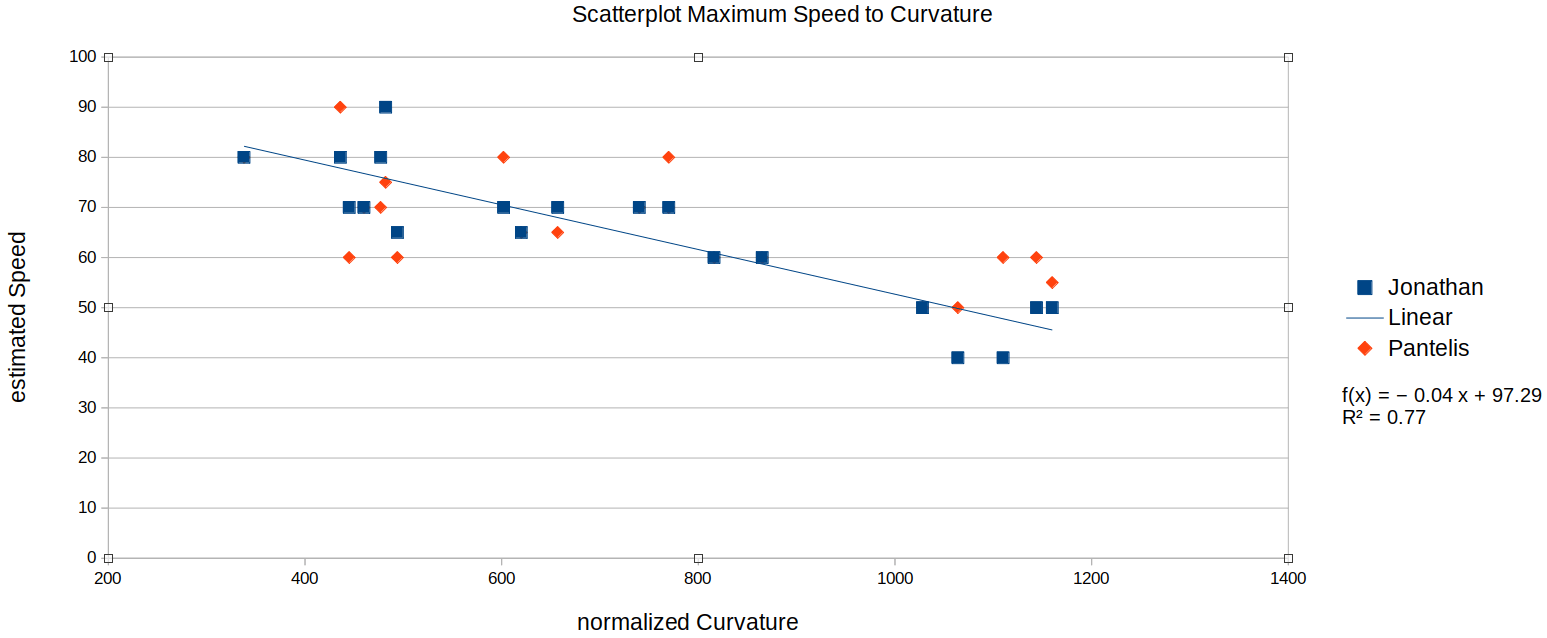
\includegraphics[width=1.0\linewidth]{images/regression.png}
    \caption{A regression for preferred speed and road curvature, see estimated\_maxV.ods.}
    \label{fig:regressionPrefspeed}
\end{figure}

    \begin{table}
    \centering
    \begin{tabular}{@{}llr@{}} \toprule
    \multicolumn{3}{r}{Preferred Speed}             \\ \cmidrule(l){2-3}
        Curvature range & [km/h] & [tiles/time-step]        \\ \midrule
        (0,200)         & 85        & 8 \\
        (200,500)       & 75        & 7 \\
        (500,900)       & 65        & 6 \\
        (900,1200)      & 54        & 5 \\
        (1200,1500)     & 40        & 4 \\
        (1500, 1900)    & 30        & 3 \\
        (1900, 10000)   & 15        & 2 \\ \bottomrule
    \end{tabular}
    \caption{A mapping between a range of curvatures and preferred speed of motorcyclists.} 
    \label{tab:dictPrefspeed}
    \end{table}
The outcome of the regression analysis was utilized to establish a correlation between a range of curvature values and preferred speed, as demonstrated in Table \ref{tab:dictPrefspeed}. The division of the curvature ranges was made in an arbitrary manner with the aim of ensuring that all speeds of a motorcyclist correspond to a specific curvature range and taking into account the distribution of the curvature values in the data\footnote{see: Curvature\_maxV.ods}. The maximum allowed speed is usually established by incrementing the preferred speed of a motorcyclist by one unit of time-step, allowing cars to maintain a faster pace relative to motorcycles.

\section{Fun Metric}
\label{sec:Fun Metric}
The fun of the motorcyclist is modeled using a standard normal distribution, taking into account their preferred speed given the curvature and desired distance from their platoon members. For each time-step, the distance to other motorcyclists and current speed are evaluated based on three standard distributions: one for the distance to the motorcyclist ahead, one for the distance to the motorcyclist behind, and one for speed. In the case of the sweeper or leader missing a partner in front or behind, one side will be duplicated. The riders who got lost will not have anything added to their fun measure for that time-step. \\
Further since a motorcyclist visits the Black Forest region for its curves (ignoring the scenic view), the enjoyment of riding through curves is weighted differently. Curves in the range of (0,400) are weighted by 0.25, while curves in the range of (400, 1000) are weighted by 1.\\
As the normal distribution is symmetric and has its highest peak at the center, this means that for an optimal scenario, where the motorcyclist is in the middle of the platoon and all distances and speeds are at their preferred levels, the value obtained by the motorcyclist would be three times the value of the highest peak of the normal distribution. However, any deviations from the desired distance or speed would result in reduced values, as the sum of normal distributions still follows a normal distribution pattern, with its peak centered around its mean\footnote{see https://en.wikipedia.org/wiki/Sum\_of\_normally\_distributed\_random\_variables, 20.02.23}. Figure \ref{fig:fun_distribution_clear_road} displays the mean fun-distribution diagram for a platoon of five motorcyclists on an empty road with a curvature of 600 for 50 time-steps. Biker 0 is designated as the initial leader, and Biker 4 is the initial sweeper. The plot shows that it takes approximately 15 time-steps for the platoon to reach its optimal distance to each other, as evidenced by the plateau of about 1.2 in the fun-distribution curve. Note that this value is about three times higher than the peak of a standard normal distribution, which is around around 0.4.\\

\begin{figure}
    \centering
    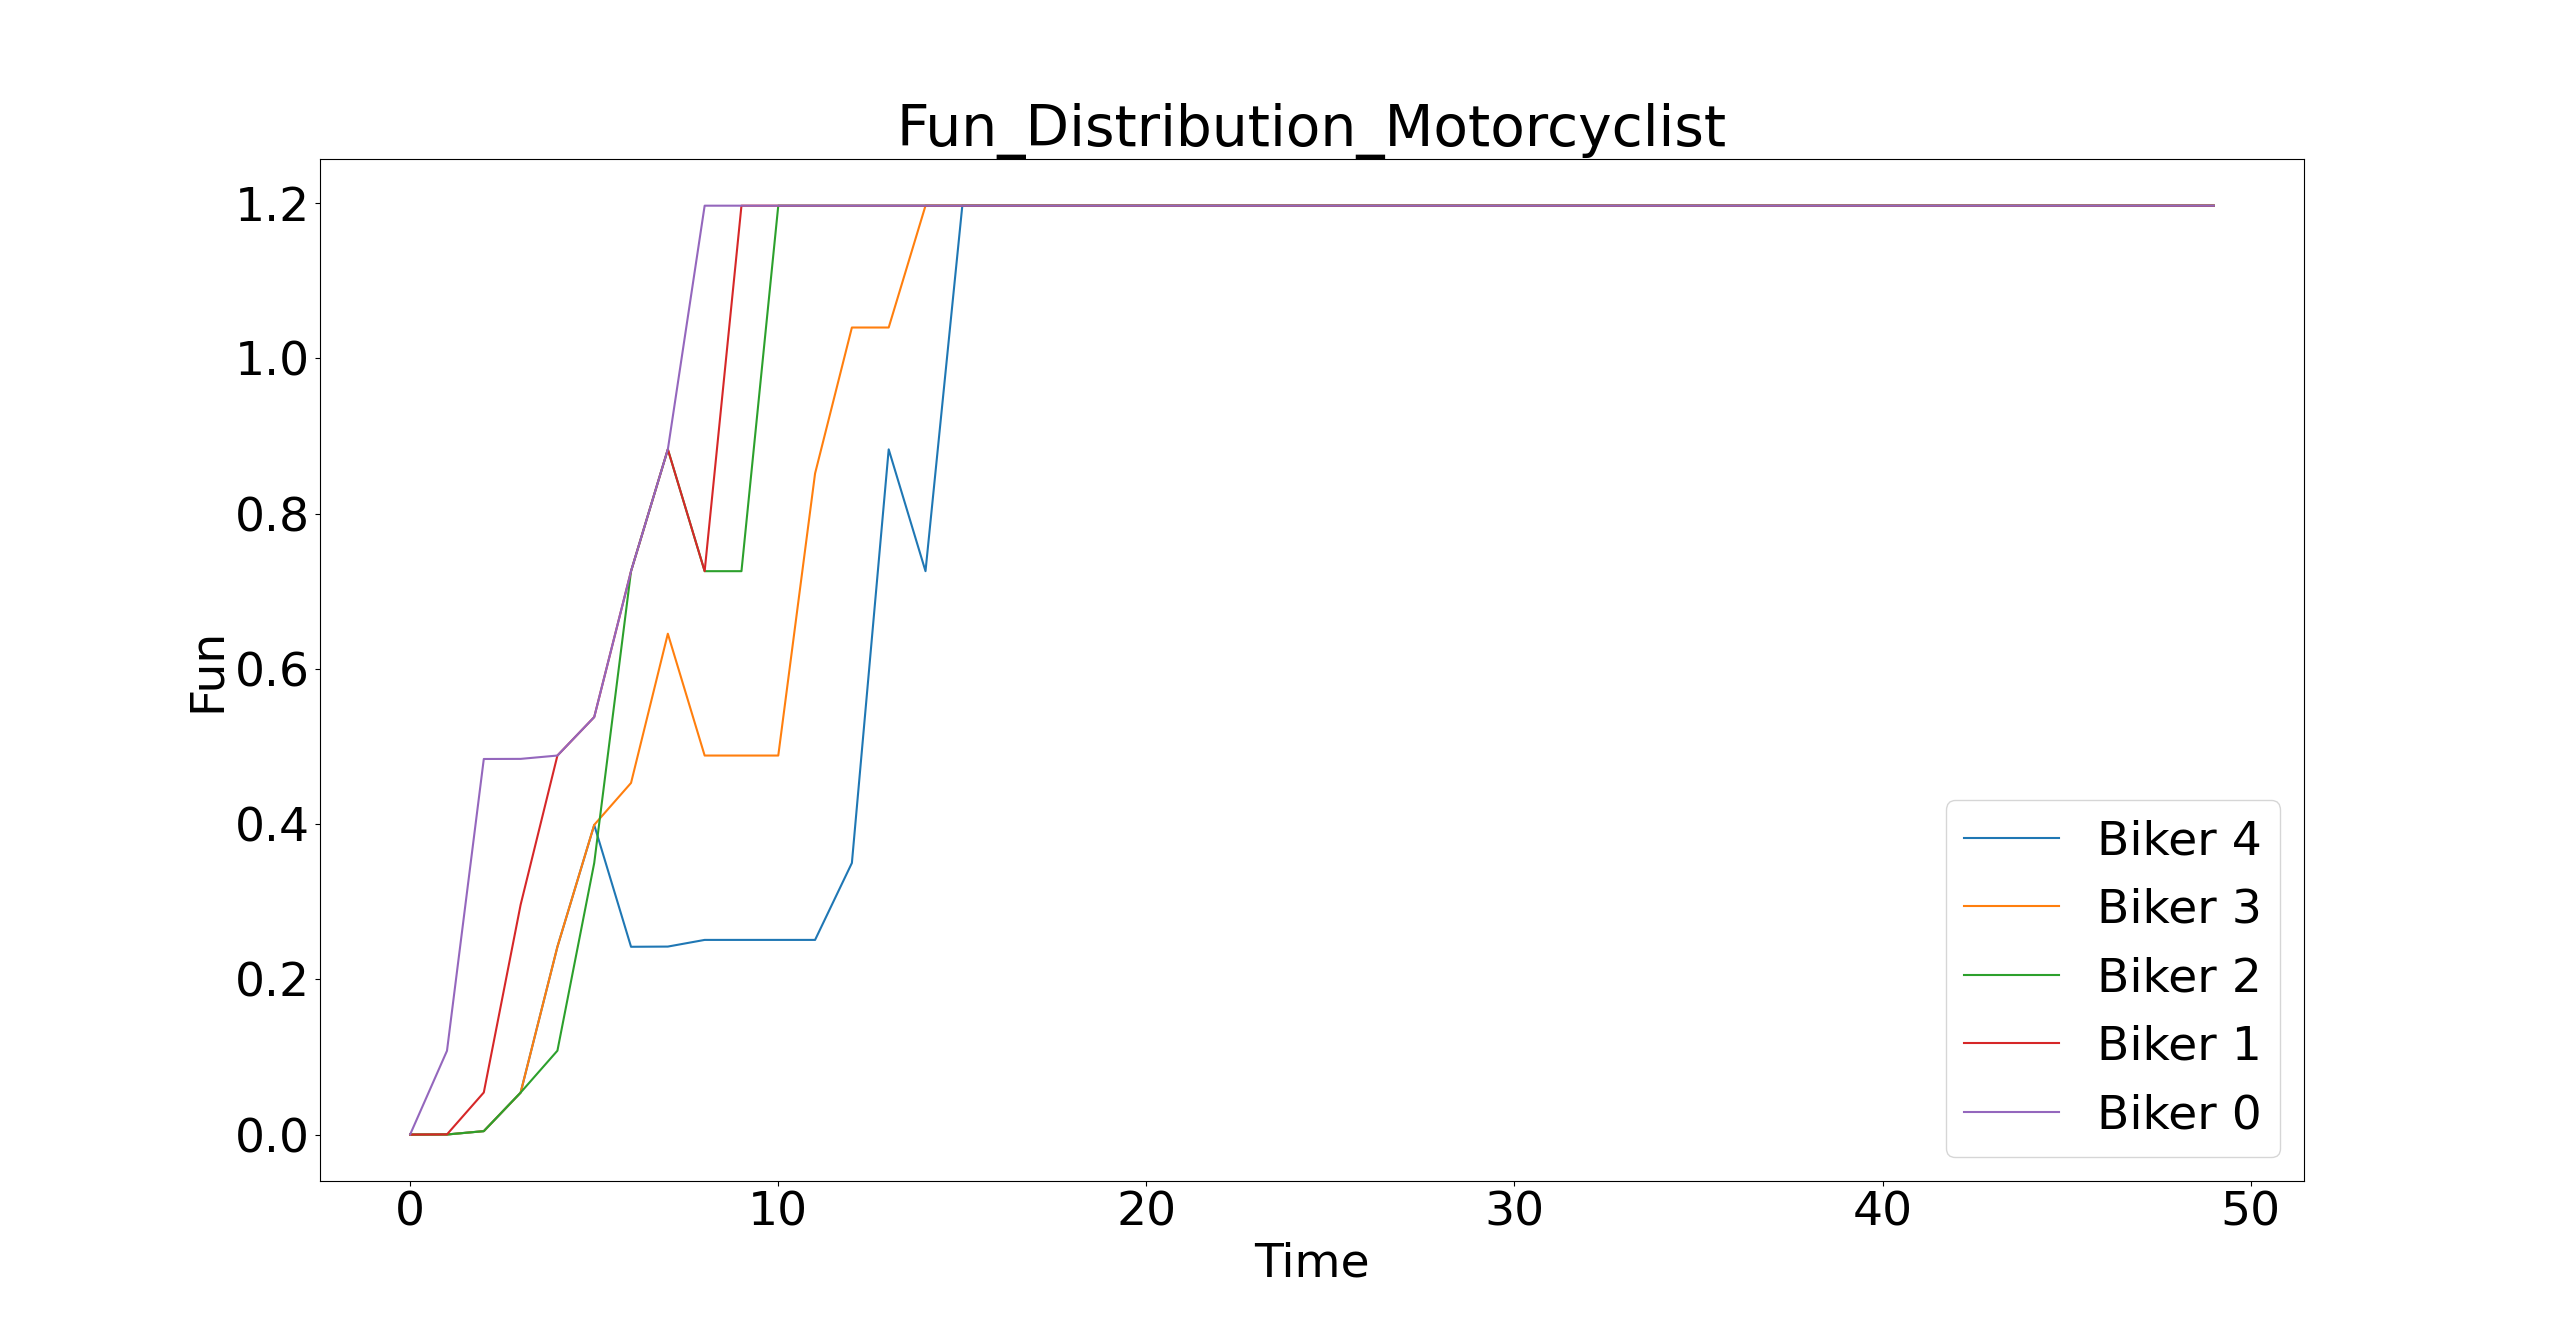
\includegraphics[width=1.0\linewidth]{images/fun_distribution_free_road.png}
    \caption{Fun-distribution of five motorcyclists on a clear road with curvature 600 for 50 time-steps, with Biker 0 as initial leader and Biker 4 as initial sweeper.}
    \label{fig:fun_distribution_clear_road}
\end{figure}

As the fun metric is based on a standard normal distribution, this indicates that the motorcyclist evaluates the preferred distance and desired speed equally. However, according to the fixed rule set, the motorcyclist prioritizes optimizing their distance to the rear platoon member, followed by their distance to the front platoon member, and finally their speed, within the platoon. A previous attempt to modify the rule set solely for maximizing the fun measure was abandoned due to coding issues and potential logical inconsistencies.



\section{Additional Metrics and Parameters}
\label{sec:Additional Metrics and Parameters}
Table \ref{tab:moreparameters} lists additional parameters of the model important for the analysis of metrics listet in table \ref{tab:moremetrics}

    \begin{table}
    \centering
    \begin{tabular}{@{}llr@{}} \toprule
        Parameter                   & Unit          & Explanation        \\ \midrule
        $length$                    & tile          & the length of the street \\
        $total\_amount\_steps$        & sec           & time the model has been running \\
        $density$                   & [0,2]         & percentage of vehicles on the road \\
        $car\_share$                 & [0,1]         & share of cars among vehicles (excluding motorcycles) \\
        $number\_platoons$           & int           & number of platoons \\
        $platoon\_size$              & int           & size of a platoon \\ \bottomrule
    \end{tabular}
    \caption{Overview of additional model parameters.} 
    \label{tab:moreparameters}
    \end{table}


    \begin{table}
    \centering
    \begin{tabular}{@{}llr@{}} \toprule
        Parameter                   & Unit                      & Explanation        \\ \midrule
        $fun$                       & float                     & see section \ref{sec:Fun Metric} \\
        $flow$                      & vehicles/time-step        & number of vehicles passing through \\
        $time\_distance$             & tiles                     & traveling distance of bikers\\
        $velocity$                  & tiles/time-step           & traveling velocity of bikers\\
        $lane$                      & left/right lane           & side of the lane \\
        $role$                      & sweeper/inbetween/leader  & role of biker in the platoon\\
        $distance\_to\_partner$       & tiles                     & distance to partner \\ \bottomrule
    \end{tabular}
    \caption{Overview of metrics used for this analysis.} 
    \label{tab:moremetrics}
    \end{table}


The flow of the two-lane traffic is defined as equation \ref{eq:model_flow}
\begin{equation}
    flow = \frac{1}{T}\sum_{lane=0}^{lane=1}\sum_{t={0}}^{T}(n_{i, i+1})
    \label{eq:model_flow}
\end{equation}
The flow of the two-lane traffic is measured as the sum of the number of vehicles that pass between $tile[0]$  and $tile[maxV]$ at time step $t$ averaged by the total number of time steps T ($total\_amount\_steps$). $n_{i, i+1}(t) = 0(1)$ indicates whether or not a vehicle has passed between those tiles at time step $t$. The flow ranges therefore between [0,2] since it accounts for both lanes. It is important to note that the flow measure does not account for the varying maximum speeds of different vehicles. As a result, it may produce unexpected or inaccurate results in situations where there is a high density of vehicles with varying maximum speeds or if the overall traffic is moving at lower speeds\footnote{Unfortunately, this issue was not detected until a very late stage of the thesis.}. This issue is discussed further in chapter \ref{chapter:Influence of model parameters on metrics}.\\
The $time\_distance$ metric is a metric in measuring the total distance covered by the platoon during a single trip. This information can be useful in identifying any brakes or gaps within the group, and it also gives insight into the progress made during the journey.\\
The $velocity$ metric provides an indication of the average speed at which a motorcyclist operates within the platoon. The influence of the leader or sweeper on this metric, given the defined rule set, will be analyzed in Chapter \ref{chapter:Influence of model parameters on metrics}.\\
The $lane$ metric provides insights into the frequency of lane changes made by a motorcyclist within a platoon. In low traffic density scenarios, it is expected that the platoon will successfully maneuver to the right lane. However, at high traffic densities, when all vehicles strive to change to the right lane, the right lane becomes congested, leading the platoon to remain on the left lane. With an increase in traffic density, the coherence of the platoon may decrease, as some members may succeed in switching to the right lane but become trapped between vehicles, while the rest of the platoon moves ahead on the left lane.\\
The $role$ metric captures the changes in the position of a motorcyclist within the platoon, as defined by the rule set. This metric allows one to observe how the role of a motorcyclist changes during the course of a trip, as they are permitted to transition from a sweeper, to an in-between rider, and finally eventually to a leader.\\
The $distance\_to\_partner$ metric provides information on the ability of bikers to maintain their distances from each other throughout the trip. It is related to the previously mentioned $fun\_measure$, but offers a more concise insight into group cohesion.


